\subsubsection*{6. Bestem stigetiden tr}
Bestem stigetiden tr (10-90).
Stigetiden er den tid det tager $V_{out}$ at komme fra 10\%  til 90\% af den statiske værdi.

Den statiske værdi defineres som $V_{stat} = 5 V$

Ved 10k$\Omega$:
\begin{equation}
	t_{10} = V_{stat\_10}\cdot 0.1 = 0.5\ V
	\label{t_10K_10}
\end{equation}

\begin{equation}
	t_{90} = V_{stat\_10}\cdot 0.9 = 4.5\ V
	\label{t_10K_90}
\end{equation}

Nu hvor begge værdier til 10\% og 90\% af den statiske værdi er kendte, kan der indsættes cursorer på grafen og derved beregne stigetiden

\begin{figure}[h]
 \begin{center}
  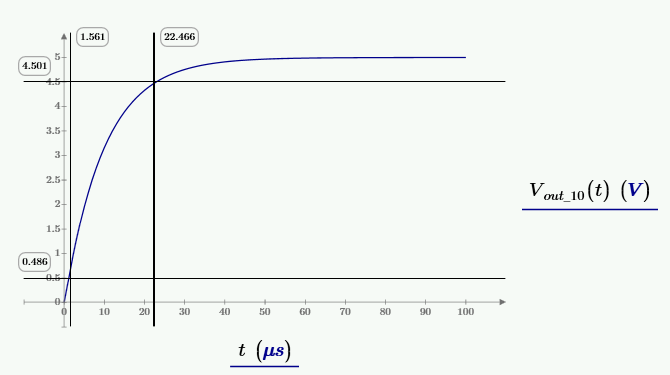
\includegraphics[height=5cm]{P_Fig/figur18_anast10K}
  \caption{stigetiden $t_r$ for 10k$\Omega$}
  \label{st10K}
 \end{center}
\end{figure}

Her aflæses:
\begin{center}
\begin{minipage}{.2\linewidth}
10\% af $V_{stat}$ er 1.561 $\mu$s,
\end{minipage} 
\begin{minipage}{.2\linewidth}
90\% af $V_{stat}$ er 22.466 $\mu$s
\end{minipage} 
\end{center}

\begin{equation}
	t_{r\_10} = t_{90}-t_{10} = 20.905\ \mu s
\end{equation}

Stigetiden for 10 k$\Omega$ er altså 20,905 $\mu$s

Ved 1k$\Omega$ vil $t_{10}$ (Ligning \ref{t_10K_10} og $t_{90}$ (Ligning \ref{t_10K_90} være det samme, da de begge har den samme stationære værdi.

Nu hvor begge værdier til 10\% og 90\% af den statiske værdi er kendte, kan der indsættes cursorer på grafen og derved beregne stigetiden

\begin{figure}[h]
 \begin{center}
  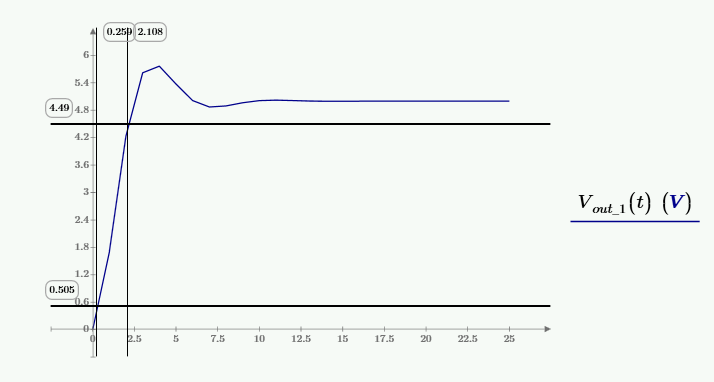
\includegraphics[height=5cm]{P_Fig/figur19_ana2st1K}
  \caption{stigetiden $t_r$ for 1k$\Omega$}
  \label{stigetid1K}
 \end{center}
\end{figure}

Her aflæses:
\begin{center}
\begin{minipage}{.2\linewidth}
10\% af $V_{stat}$ er 0.259 $\mu$s,
\end{minipage} 
\begin{minipage}{.2\linewidth}
90\% af $V_{stat}$ er 2.108 $\mu$s
\end{minipage} 
\end{center}

\begin{equation}
	t_{r\_1} = t_{90}-t_{10} = 1.849\ \mu s
\end{equation}

Stigetiden for 1 k$\Omega$ er altså 1.849 $\mu$s